\documentclass[conference]{IEEEtran}
\IEEEoverridecommandlockouts
% The preceding line is only needed to identify funding in the first footnote. If that is unneeded, please comment it out.
\usepackage{cite}
\usepackage{amsmath,amssymb,amsfonts}
\usepackage{algorithmic}
\usepackage{graphicx}
\usepackage{textcomp}
\usepackage{xcolor}
\usepackage{tabularx}
\usepackage{multirow}
\usepackage{graphics} % for pdf, bitmapped graphics files
\usepackage{subfig}
\usepackage{subcaption}
\usepackage{hyperref}
\usepackage{academicons}
\usepackage{xcolor}
\usepackage{listings}
\usepackage{tabularx} % Asegúrate de incluir este paquete

\usepackage{tikz}
\usetikzlibrary{shapes.geometric, arrows}

\usetikzlibrary{shapes.geometric, arrows}

\tikzstyle{startstop} = [rectangle, rounded corners, minimum width=3cm, minimum height=1cm,text centered, draw=black, fill=red!30]
\tikzstyle{process} = [rectangle, minimum width=3cm, minimum height=1cm, text centered, draw=black, fill=blue!30]
\tikzstyle{arrow} = [thick,->,>=stealth]


\def\BibTeX{{\rm B\kern-.05em{\sc i\kern-.025em b}\kern-.08em
		T\kern-.1667em\lower.7ex\hbox{E}\kern-.125emX}}

% Color Enlace
\definecolor{colorEnlace}{RGB}{0, 0, 0}
\hypersetup{
	colorlinks=true,
	linkcolor=colorEnlace,
	citecolor=colorEnlace,
	urlcolor=colorEnlace,
	pdfauthor={Davis Bremdow Salazar Roa},
	pdftitle={Sistemas digitales a tener en cuenta}
}

\definecolor{mybg}{rgb}{0.97,0.97,0.97}
\definecolor{mygray}{gray}{0.4}
\definecolor{mygreen}{rgb}{0,0.6,0}
\definecolor{myblue}{rgb}{0,0,0.8}
\definecolor{mypurple}{rgb}{0.58,0,0.82}
\definecolor{myred}{rgb}{0.7,0,0}

\lstdefinelanguage{MatlabEnhanced}{
	language=Matlab,
	morekeywords={[2]linspace,plot,title,xlabel,ylabel,legend,grid},
	morekeywords={[3]sin,cos,exp,log,sqrt},
	keywordstyle=\color{myblue}\bfseries,
	keywordstyle=[2]\color{mypurple},
	keywordstyle=[3]\color{myred},
	commentstyle=\color{mygreen}\itshape,
	stringstyle=\color{mygray},
	morecomment=[l]%
}

\lstset{
	language=MatlabEnhanced,
	backgroundcolor=\color{mybg},
	frame=single,
	basicstyle=\ttfamily\small,
	showstringspaces=false,
	numbers=none,              %
	xleftmargin=0pt,           %
	framexleftmargin=0pt,      
	framexrightmargin=0pt,
	framextopmargin=2pt,
	framexbottommargin=2pt,
	breaklines=true,
	tabsize=1,
}

% Control 
\usepackage{amsmath}
\begin{document}
	
	\title{Circuitos Mezcladores}
	\author{
		\makebox[\textwidth][c]{\large\textbf{Universidad Nacional de San Antonio Abad del Cusco}}\\
		\makebox[\textwidth][c]{\normalsize\textit{Escuela profesional de Ingeniería Electrónica}}\\
		\makebox[\textwidth][c]{\normalsize\textit{Ingeniero Antero Casani}}\\
		\makebox[\textwidth][c]{\normalsize\textit{Circuitos Electrónicos III}}\\
		\and
		\IEEEauthorblockN{Yency Manuel Huamanga Chumbes}
		\IEEEauthorblockA{ Estudiante de Ingeniería Electrónica \\
			Cusco, Perú \\
			171864@unsaac.edu.pe}
		\and
		\IEEEauthorblockN{Ruth Juana Espino Puma}
		\IEEEauthorblockA{Estudiante de Ingeniería Electrónica \\
			Cusco, Perú \\
			184657@unsaac.edu.pe}
		\and
		\IEEEauthorblockN{Davis Bremdow Salazar Roa}
		\IEEEauthorblockA{Estudiante de Ingeniería Electrónica \\
			Cusco, Perú \\
			200353@unsaac.edu.pe}
	}
	
	\maketitle
	\begin{abstract}
		En este trabajo se estudian los mezcladores de frecuencia, su funcionamiento, tipos, circuito de aplicacion y analisis de simulacion.
	\end{abstract}
	\begin{IEEEkeywords}
		Mezclador, frecuencia intermedia, RF, suma y diferencia.
	\end{IEEEkeywords}
	%% Contenido del documento
	
	% Circuito y simulación
	
	\section{Circuito Mezclador}
	
	Dentro de la clasificación de los circuitos mezcladores, existen diferentes aplicaciones para cada una de ellas, sin embargo dentro del ámbito de las telecomunicaciones las principales se centrar en los circuitos RF (Radio Frecuencia) y cuyo análisis es de interés para comprender como es posible la propagación de información en forma de onda electromagnética, en la figura \ref{fig:circuito-mezclador} se puede apreciar un circuito receptor superheterodino el cual se encargará de multiplicar una señal de entrada con la generada por un oscilador local para su desplazamiento en frecuencia, logrando de tal forma la recepción de una señal de información.
	
	\begin{figure}[h]
		\centering
		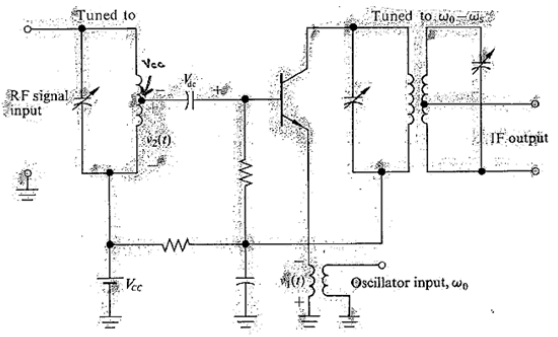
\includegraphics[width=0.5\textwidth]{media/circuito-mezclador}
		\caption{Circuito Mezclador - Transistor Bipolar}
		\label{fig:circuito-mezclador}
	\end{figure}
	
	Teniendo en cuenta este circuito se puede modelar un ejemplo para la obtención de sus parámetros el cual se describe a continuación:
	
	Considere un mezclador bipolar del tipo mostrado en la Fig. 7.2-3. Suponiendo que la componente DC de la corriente de emisor es de 1 mA y que el voltaje pico de excitación del oscilador (a través del lado del emisor del transformador de excitación) es de 100 mV, determine Gc y Gm. Asumiendo que la señal de entrada tiene una amplitud pico de 2 mV, evalúe los componentes de corriente en el colector para la frecuencia de la señal de entrada, la frecuencia del oscilador y la frecuencia de diferencia.
	
	\textbf{Datos del problema}
	
	\begin{itemize}
		\item Corriente DC: $I_E = 1mA$
		\item Señal del oscilador: $V_1 = 100V$ (Pico)
		\item Señal de entrada: $V_2 = 2v$ (Pico)
	\end{itemize}
	
	\subsection{Solución}
	
	Sabemos que la corriente del emisor es:
	
	\begin{equation}
		i_{E}(t) = I_{E}e^{v(t)/V_{T}}, \quad \text{donde } v(t) = V_{1}\cos(\omega_{0}t) + V_{2}\cos(\omega_{s}t)
	\end{equation}
	
	Definimos:
	
	\begin{equation}
		x = \frac{V_{1}}{V_{T}} = \frac{0,1}{0,025} = 4, \qquad y = \frac{V_{2}}{V_{T}} = \frac{0,002}{0,025} = 0,08
	\end{equation}
	
	Los términos relevantes para la señal de entrada y productos de mezcla son:
	
	\begin{equation}
		G_{m} = \frac{2I_{E}I_{0}(x)I_{1}(y)}{V_{2}}, \qquad G_{c} = \frac{4I_{E}I_{1}(x)I_{1}(y)}{V_{2}}
	\end{equation}
	
	Usando:
	
	\begin{equation}
		I_{0}(4) \approx 11,3019, \quad I_{1}(4) \approx 9,7595, \quad I_{1}(0,08) \approx 0,04
	\end{equation}
	
	Para obtener una valor exacto entre las corrientes fue necesario cuantizar los valores en función x, tales valores se obtienen a partir de la tabla que se muestra en \cite{pozar2011mixers} y la cual se muestra en la figura \ref{fig:valores-corriente}
	
	\begin{figure}[h]
		\centering
		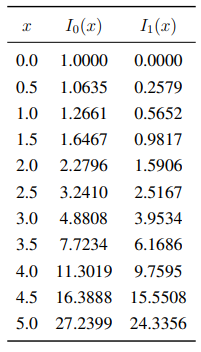
\includegraphics[width=0.4\textwidth]{media/valores-corriente}
		\caption{Tabla de valores $I_0(x), I_1(x)$}
		\label{fig:valores-corriente}
	\end{figure}
	
	Finalmente con estos valores se obtiene, la transconductancia amplificadora, conversión y los componentes de corriente colector, estas relaciones se puede aprec
	
	
	
	\begin{equation}
		G_m = \frac{2*1*11.3019*0.04}{0.002} = 452.08m\frac{A}{V}
	\end{equation}
	
	
	\begin{equation}
		G_c = \frac{4*1*9.7595*0.04}{0.002} = 1.5615m\frac{A}{V}
	\end{equation}
	
	
	\begin{equation}
		i_C(\omega_s) = G_m V_2 = 452,08 \cdot 0,002 = 0.904mA
	\end{equation}
	
	\begin{equation}
	i_C = G_c \cdot V_2 = 780,76 \cdot 0,002 = 1.561mA
	\end{equation}
	
	Finalmente de los resultados obtenidos se puede apreciar la capacidad de los mezcladores para la amplificación de los productos cruzados entre las señales de operación lo cual es un punto de vital importancia para el funcionamiento de los sistemas de comunicación.
	
	% FM
	
	\section{Circuitos Mezcladores en la modulación FM}
	
	\subsection{Circuito Modulador FM}
	
	Dentro de las aplicaciones aplicadas a la radio frecuencia además de los circuitos mezcladores anteriormente mostrados, otra de poder implementar físicamente un mezclador para una modulación FM es mediante el empleo del circuito integrado XR2206 el cual es un generador de señales (sinusoidales, cuadradas y triangulares) según la configuración entre sus pines y las salidas a usar, un esquema genera sobre este integrado se puede obtener en su hoja de datos en la cual se detallan ejemplos y especificaciones sobre su funcionamiento.
	
	\begin{figure}[h]
		\centering
		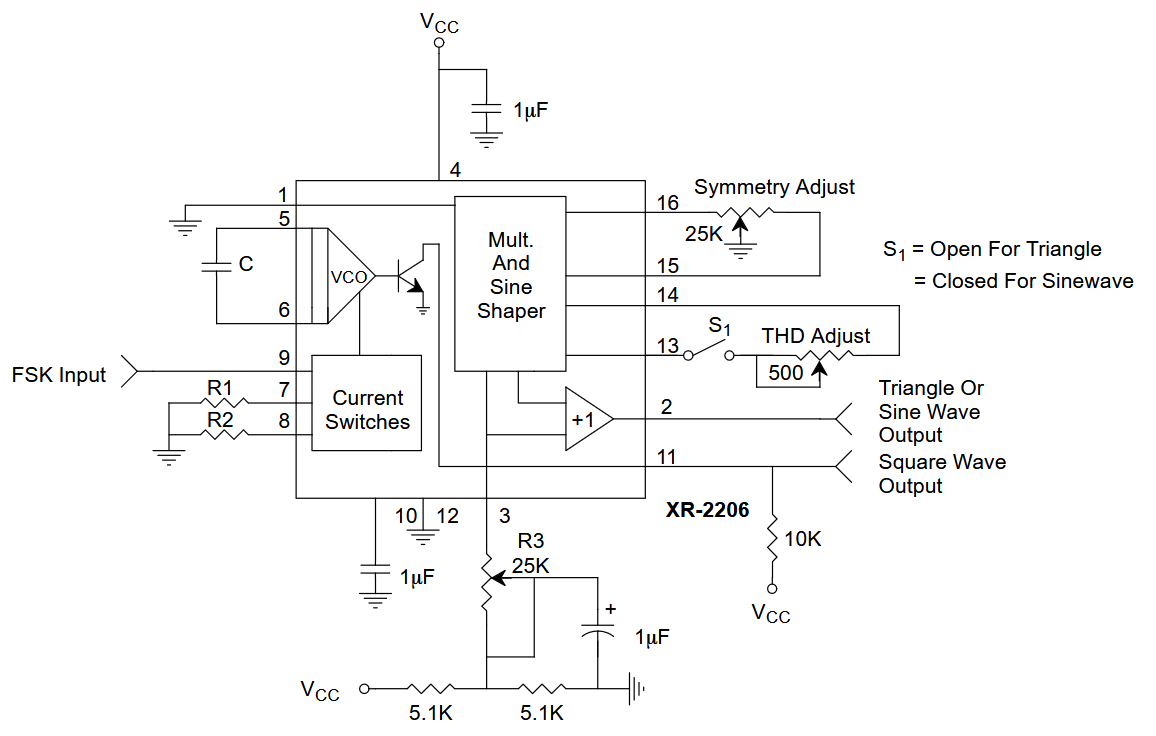
\includegraphics[width=0.5\textwidth]{media/integrado-xr2206}
		\caption{CI - Generador de señales XR2206}
		\label{fig:integrado-xr2206}
	\end{figure}
	
	En la figura \ref{fig:integrado-xr2206} se puede apreciar un esquema gráfico con una configuración inicial elegida para su funcionamiento como oscilador o generador de señales.
	
	Sin embargo si se desea tener un mayor control de la frecuencia de la señal generada el diagrama general del CI en la figura \ref{fig:diagrama-bloques-xr2206} muestra la configuración de pines, siendo los de relevancia los pines 5 y 6 (conexión para el capacitor) y 7 y 8 (pines para la resistencia) los cuales definen la frecuencia de oscilación del circuito bajo la ecuación que se define en \ref{eq:frecuencia-oscilacion} y utilizando el resto de pines para la polarización y salidas.
	
	Otra configuración a tener en cuenta corresponde a la amplitud de la portadora, la cual se puede configurar según la hoja de datos mediante la conexión entre los pines 13 y 14 para una señal senoidal y como un circuito abierto para el empleo de una señal triangulo, esta configuración a mayor detalle se aprecia en la figura \ref{fig:integrado-xr2206}, siendo necesario para modificar el valor de la resistencia entre ambos pines para modificar la amplitud la cual tiene una correspondencia proporcional entre el voltaje de salida respecto a la amplitud, donde se puede apreciar que se tendrá una salida de $a = \frac{60mV}{K\Omega}$, donde \textbf{a} representa la amplitud de la señal generada por el CI.
	
	\begin{equation}
		\omega_o = \frac{1}{CR}
		\label{eq:frecuencia-oscilacion}
	\end{equation}
	
	
	Una vez definidos los parámetros para el funcionamiento del CI, es posible tener un ejemplo sobre el funcionamiento del mismo mediante NI Multisim y en el cual este circuito se configurara de forma que sirva como un modulador FM mediante el empleo de una señal moduladora originada por el generador de funciones.
	
	\begin{figure}[h]
		\centering
		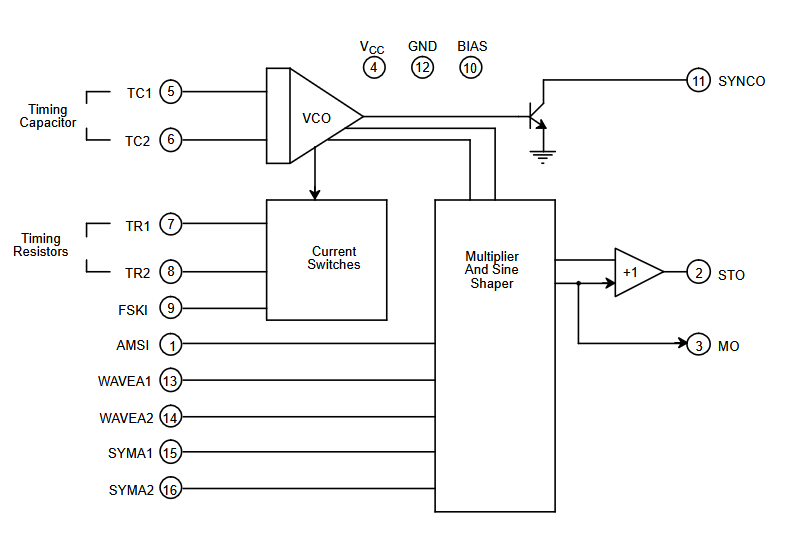
\includegraphics[width=0.5\textwidth]{media/diagrama-bloques-xr2206}
		\caption{Diagrama de bloques del CI XR2206}
		\label{fig:diagrama-bloques-xr2206}
	\end{figure}
	
	Un ejemplo de esta implementación se puede apreciar en la figura \ref{fig:simulacion-xr2206} en la cual se muestran los componentes antes mencionados para una frecuencia de la portadora de 1K Hz la cual responde a la inversa del producto de la capacitancia y resistencia según \ref{eq:frecuencia-oscilacion}.
	
	Mientras que el tono de información se configuro con una frecuencia de 100 Hz con un amplitud $V_{pp} = 20V$, la cual se acoplo al circuito integrado mediante un divisor de tensión al pin 7.
	
	
	\begin{figure}[h]
		\centering
		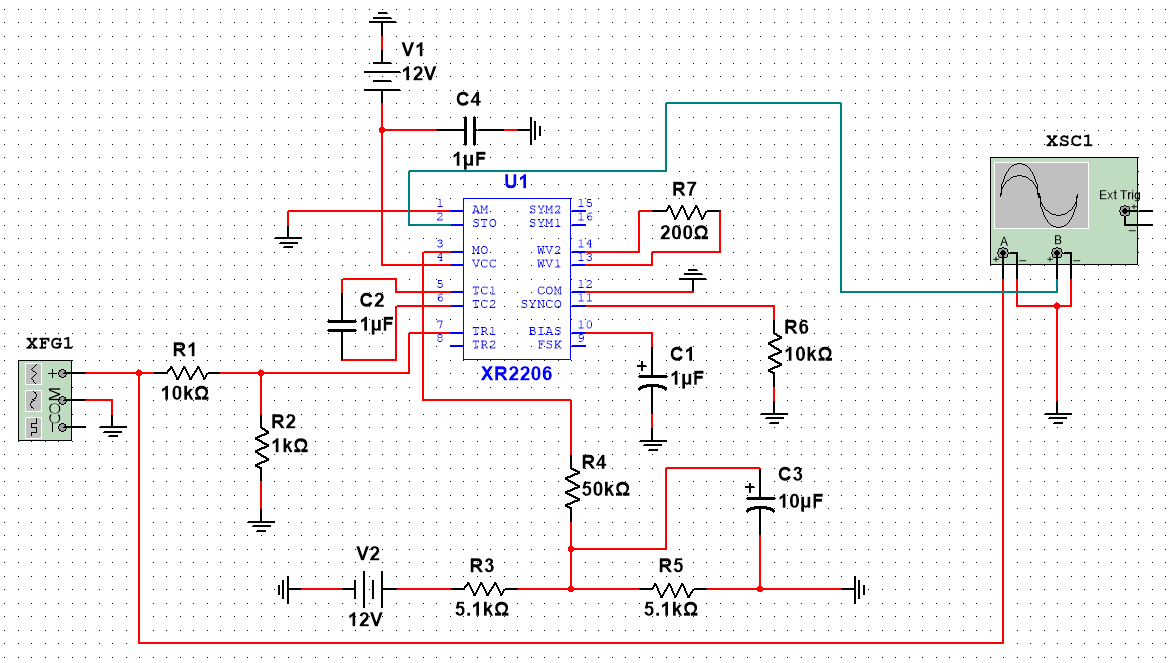
\includegraphics[width=0.5\textwidth]{media/simulacion-xr2206}
		\caption{Circuito Modulador FM - NI Multisim}
		\label{fig:simulacion-xr2206}
	\end{figure}
	
	Finalmente para la visualización de las señales se hizo uso de un osciloscopio de 2 entradas y en la cual se aprecia en su primer terminal la señal de información y en el segundo la señal FM generada a partir del CI XR2206 y mediante la cual se pudo apreciar las variaciones de frecuencia.
	
	\section{Señal FM generada}
	
	Mediante el empleo del osciloscopio se puede apreciar la forma de onda de salida del circuito integrado la cual al compararla con la señal sinusoidal de entrada se puede apreciar los cambios de frecuencia para la excursión positiva de la señal como se muestra en la figura \ref{fig:mod-fm-circuito}.
	
	\begin{figure}[h]
		\centering
		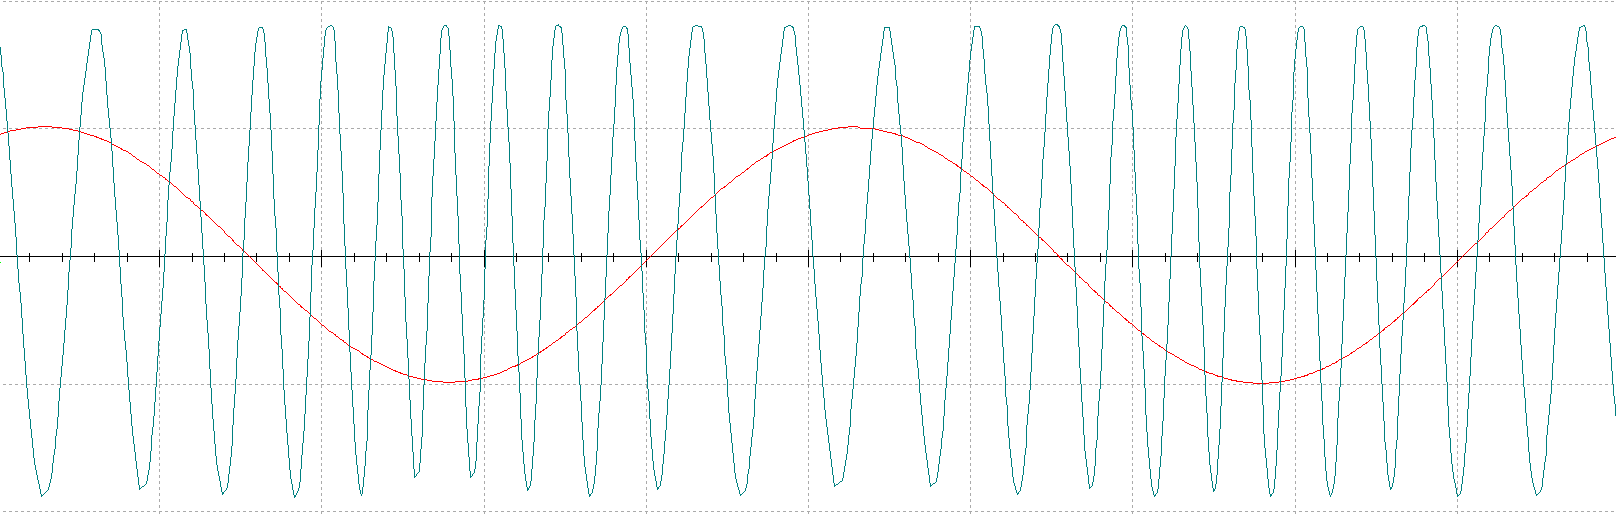
\includegraphics[width=0.5\textwidth]{media/mod-fm-circuito}
		\caption{Modulación FM - Circuito Integrado XR2206}
		\label{fig:mod-fm-circuito}
	\end{figure}
	
	Por otro lado si se considera una mayor frecuencia (400 [Hz]) en la moduladora, la señal de salida presenta cambios menos significativos en la señal, ello debido a que las variaciones de frecuencia son muy próximas a la frecuencia de la portadora, este efecto puede limitar la modulación debido a que se tendría una mezcla de señales muy parecida, este efecto se muestra en la figura \ref{fig:mod-fm-circuito-400}
	
	\begin{figure}[h]
		\centering
		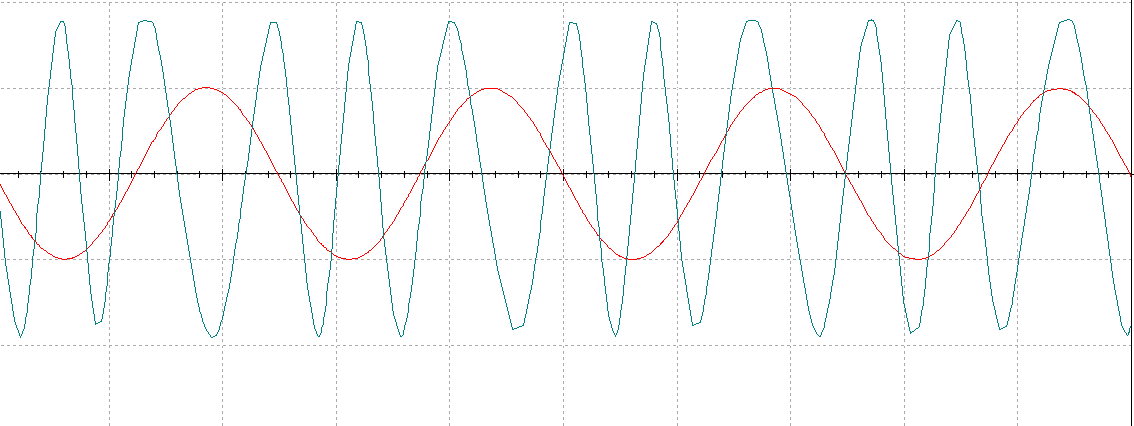
\includegraphics[width=0.7\textwidth]{media/mod-fm-circuito-400}
		\caption{Modulación FM de un tono - Circuito Integrado XR2206}
		\label{fig:mod-fm-circuito-400}
	\end{figure}
	
	El comportamiento previamente explicado se puede justificar mediante la expresión general de una señal FM definida en \ref{eq:mod-fm}, la cual se menciona en \cite{stremler2006}
	
	\begin{equation}
		\phi_{FM}(t) = Asin( \omega_c t + \int_0^t k_f f(\tau)\, d\tau + \theta_0\ )
		\label{eq:mod-fm}
	\end{equation}
	
	Y mediante la cual se aprecia que si la señal de la moduladora es próxima a la frecuencia de la señal portadora, estas se aproximan entre si generando pequeños cambios que dependerán completamente del indice de modulación.
	
	\bibliographystyle{IEEEtran}
	\bibliography{biblio}
	
	
	
\end{document}